\chapter{Analisi dei dati}
\bigskip

\section{Wikipedia}
\bigskip
Wikipedia (\url{https://wikipedia.org}) è un enciclopedia online, a contenuto libero e gratuito, lanciata da Jimmy 
Wales e Lerry Sangers nel 2001 ed ora gestita dalla Wikimedia Foundation. Al suo interno sono presenti 45 milioni di voci in 
oltre 280 lingue raggruppate in diverse \textit{categorie}. Wikipedia è il quinto sito più visitato al mondo. La sola 
versione italiana di Wikipedia (\url{http://it.wikipedia.org}) ha avuto nel 2016  una media giornaliera di 17 milioni di 
visite \cite{it_wikipedia_views_2016}; al momento in cui scriviamo (maggio 2017), conta circa 1400000 articoli 
\cite{wikipedia_stats}.
\bigskip

I dati che si andranno ad utilizzare riguardano le \textit{page view} di Wikipedia in italiano \cite{wikipedia_pageviews}. 
Con \textit{page view} si intende il numero di visite che sono state effettuate su una determinata pagina di Wikipedia in un 
certo lasso di tempo. Esse sono dati grezzi; infatti indicano il numero di visite cumulative ricevute da una voce (quindi 
anche multiple visite dello stesso utente nella stessa ora) e non distinguono tra visite effettuate da esseri umani oppure 
effettuate da bot (come i crawler). Queste informazioni sono comprensive soltanto delle visite effettuate tramite dispositivi 
desktop. Le visualizzazioni effettuate da dispositivi mobili non sono presenti all'interno delle statistiche.
\bigskip

I file di log di Wikipedia analizzati per estrarre le informazioni sono così costruiti: ogni giorno 
vengono redatti una serie di file, con cadenza oraria, in cui vengono memorizzati per ciascuna voce di ogni progetto di 
Wikipedia le visite effettuate in quell'ora. Per esempio, il file \textit{pagecounts-20071209-180000.gz} conterrà, per ogni 
voce di Wikipedia, le visite orarie del 09 Settembre 2007 effettuate dalle ore 18:00 fino alle 18:59. La struttura interna 
dei file è invece formata da quattro campi principali: una sigla identificativa del nome del progetto di Wikipedia, il nome 
della pagina, il numero di visite di quella pagina in quell'ora e la dimensione della pagina richiesta (in \textit{byte}).
\bigskip 
  
Ovviamente, ci si è focalizzati sulle \textit{page view} di specifiche pagine che sono state selezionate per essere usate 
come regressori del modello. Per ottenere un elenco di tutte le voci è stato utilizzato il tool \textit{PetScan} 
\cite{PetScan}, una web-application che permette di trovare specifici articoli, immagini, categorie che soddisfano 
determinati requisiti. La Tabella \ref{tab:ch_2_wikipedia_cat} indica le categorie da cui abbiamo ricavato le pagine 
necessarie per il progetto. Inoltre, per verificare poi la validità del modello finale, abbiamo anche estratto un altro 
dataset contente tutte le voci di alcune cateorie di Wikipedia prese in modo casuale.
\bigskip

\begin{table}[h]
\centering 
\begin{tabular}{|l|}
\hline
\rowcolor[HTML]{EFEFEF} 
\multicolumn{1}{|c|}{\cellcolor[HTML]{EFEFEF}\textbf{Dataset principale}} \\ \hline
\textit{Malattie infettive virali}                                        \\ \hline
\textit{Malattie infettive}                                                \\ \hline
\textit{Epidemie}                                                         \\ \hline
\textit{Virus}                                                            \\ \hline
\textit{Vaccini}                                                          \\ \hline
\textit{Segni clinici}                                                     \\ \hline
\end{tabular}
\quad
\begin{tabular}{|l|}
\hline
\rowcolor[HTML]{EFEFEF} 
\multicolumn{1}{|c|}{\cellcolor[HTML]{EFEFEF}\textbf{Dataset random}} \\ \hline
\textit{Investigatori immaginari}                                    \\ \hline
\textit{Aziende di abbigliamento italiane}                           \\ \hline
\textit{Software con licenza GNU LGPL}                               \\ \hline
\end{tabular}
\caption{\textit{Categorie di Wikipedia da cui sono state prese le voci per i vari dataset.}}
\label{tab:ch_2_wikipedia_cat}
\end{table}

Sono state scelte queste categorie poiché si cerca appunto una correlazione tra l'uso di Wikipedia e la percentuale di 
popolazione con patologie influenzali. Infatti, si assume che una persona malata tenda a cercare su internet, utilizzando 
motori di ricerca come Google, i propri sintomi (\textit{febbre}, \textit{influenza} o \textit{raffreddore}) e che nella 
maggior parte dei casi vada a controllare le voci di Wikipedia che trattano quei sintomi. Il dataset casuale è stato appunto 
definito per verificare che esista effettivamente questa relazione e che non sia possibile costruire modelli equivalenti 
utilizzando voci scelte a caso. Infatti, il modello dovrebbe dare risultati coerenti soltanto utilizzando il dataset che 
comprende voci di categoria medica inerenti all'influenza. 
\bigskip 

Per raffinare la lista di voci, l'elenco è stato generato sottraendo tutti gli articoli affini anche alla categoria 
\textit{Patologie aviarie}, per arrivare ad un insieme di 468 feature \cite{PetScanQuery}. Successivamente, sono state 
aggiunte le voci della \textit{Pagina_principale} (come parametro di controllo) e della voce di disambiguazione 
\textit{Influenza}, per arrivare ad un totale finale di 470 feature. Per quanto riguarda il dataset casuale, possiamo contare 
un totale di 463 voci \cite{PetScanRandom}.
\bigskip

Poiché i dati di InfluNet ci forniscono informazioni settimanali, anche i dati di Wikipedia sono stati aggregati 
settimanalmente. Il dataset totale di Wikipedia copre un arco di tempo che va dal Dicembre 2007 al Maggio 2016, per un totale 
di circa 480 settimane.

\section{Influnet}
\bigskip 

I dati riguardanti i livelli di ILI in Italia sono stati ottenuti attraverso l'analisi dei bollettini InfluNet,
che vengono pubblicati settimanalmente dal Ministero della Salute per tutta la durata del periodo influenzale.
Questi bollettini forniscono dati e statistiche dettagliate sulla diffusione e sui casi di influenza. Essi presentano 
informazioni come l'incidenza nelle varie fasce d'età o il numero di assistiti totali sottoposti a controlli. 
Questi dati vengono raccolti da diversi medici sentinella presenti su tutto il territorio nazionale (principalmente medici di medicina generale e pediatri di libera scelta).
\bigskip

Attualmente, i dati non sono disponibili in formati facilmente analizzabili (come file \textit{.csv}). Tutti i bollettini
sono in formato PDF e tutte le informazioni contenute nelle varie tabelle sono state estratte mediante l'utilizzo del software \textit{Tabula} (\url{http://tabula.technology/}). I file CSV ottenuti contengono i seguenti campi:
\begin{itemize}[noitemsep]
\item \textbf{Settimana}: coppia anno-settimana che indica la fascia temporale a cui i dati si riferiscono;
\item \textbf{Totale Medici}: totale dei medici sentinella che hanno partecipato al programma ed inviato i dati durante la settimana di riferimento; 
\item \textbf{Totale Casi}: totale dei casi di influenza rilevati;
\item \textbf{Totale Assistiti}: totale degli assistiti coperti dai medici sentinella;
\item \textbf{Incidenza Totale}: incidenza totale dell'influenza su 1000 assistiti;
\end{itemize}
\bigskip

I dati forniti da InfluNet spaziano dalla stagione influenzale 2003-2004 fino alla più recente 2016-2017. Per questo progetto 
si sono utilizzate le informazioni che comprendono la stagione influenzale 2007-2008 fino alla 2015-2016, per un totale di 
227 settimane. Per ogni stagione influenzale i dati coprono le settimane che vanno dalla numero 42 (metà Ottobre circa) fino 
alla numero 17 (metà Aprile circa dell'anno successivo). Inoltre, poiché la stagione influenzale 2008-2009 è stata più 
aggressiva rispetto agli anni precedenti (a causa del virus H1N1), in quel caso abbiamo dati fino che spaziano dall'Ottobre 
2008 fino all'Ottobre 2009.

\section{Analisi}
\bigskip

Si presentano ora alcune statistiche e grafici che forniscono maggiori informazioni riguardo alla composizione del dataset di 
Wikipedia e del dataset di Influnet, che andremo poi ad utilizzare allenare/testare il modello. Si è analizzato come 
cambia negli anni il volume totale delle visite effettuate sulle 470 voci selezionate e si è 
l'andamento delle varie stagioni influenzali.
\bigskip

In riferimento ai dati di Wikipedia, si può notare come negli anni il numero di visualizzazioni è calato drasticamente (si 
veda la Figura \ref{fig:ch_2_annual_visit}). Questo potrebbe essere spiegato dal fatto che i dati non contano gli accessi 
effettuati tramite dispositivi mobili (tablet e smartphone) che oramai stanno diventando un mezzo privilegiato per accedere 
ad internet. Infatti, da maggio 2015 il numero delle visite alle pagine di Wikipedia effettuate da dispositivi mobili ha 
superato il numero delle visite effettuate da desktop \cite{wikipedia_mobile_desktop}.
\bigskip

La voce con il maggior numero medio di visualizzazioni settimanali è quella del \textit{Virus del papilloma umano} (circa 
5560), mentre la voce \textit{Stimmate (medicina)} è quella con il numero medio minore di visualizzazioni (si parla sempre 
del periodo Dicembre 2007 - Maggio 2016); il numero medio di visite settimanali fra tutte le voci è circa 215. 
Si è analizzato il traffico di Wikipedia in italiano per comprendere da quale paese sono effettuate la maggior parte 
delle visite (per controllare se \textit{pageview} in nostro possesso siano state fatte da utenti italiani). 
Ovviamente, il 90.8\% del traffico viene effettuato dall'Italia, con punte trascurabili del 1.4\% dalla Germania, 1.0\% dagli 
Stati Uniti e di altri paesi minori \cite{WikipediaStatsCountry}.
\bigskip

Riguardo ai dati ILI, si può notare come il picco influenzale si collochi in media alla quinta settimana della stagione con 
l'unica eccezione della stagione 2009-2010 che invece ha il suo picco nella quarantaseiesima settimana (si veda la 
Figura \ref{fig:ch_2_ILI_levels}). L'incidenza delle patologie influenzali si attesta mediamente a 3.40 casi per 1000 
assistiti, mentre il picco massimo si è registrato nel 2009-2010 con 12.92 casi e il picco minimo si è verificato nella 
stagione 2015-2016 con 6.14 casi per 1000 assistiti.
\bigskip

\begin{figure}[h!]

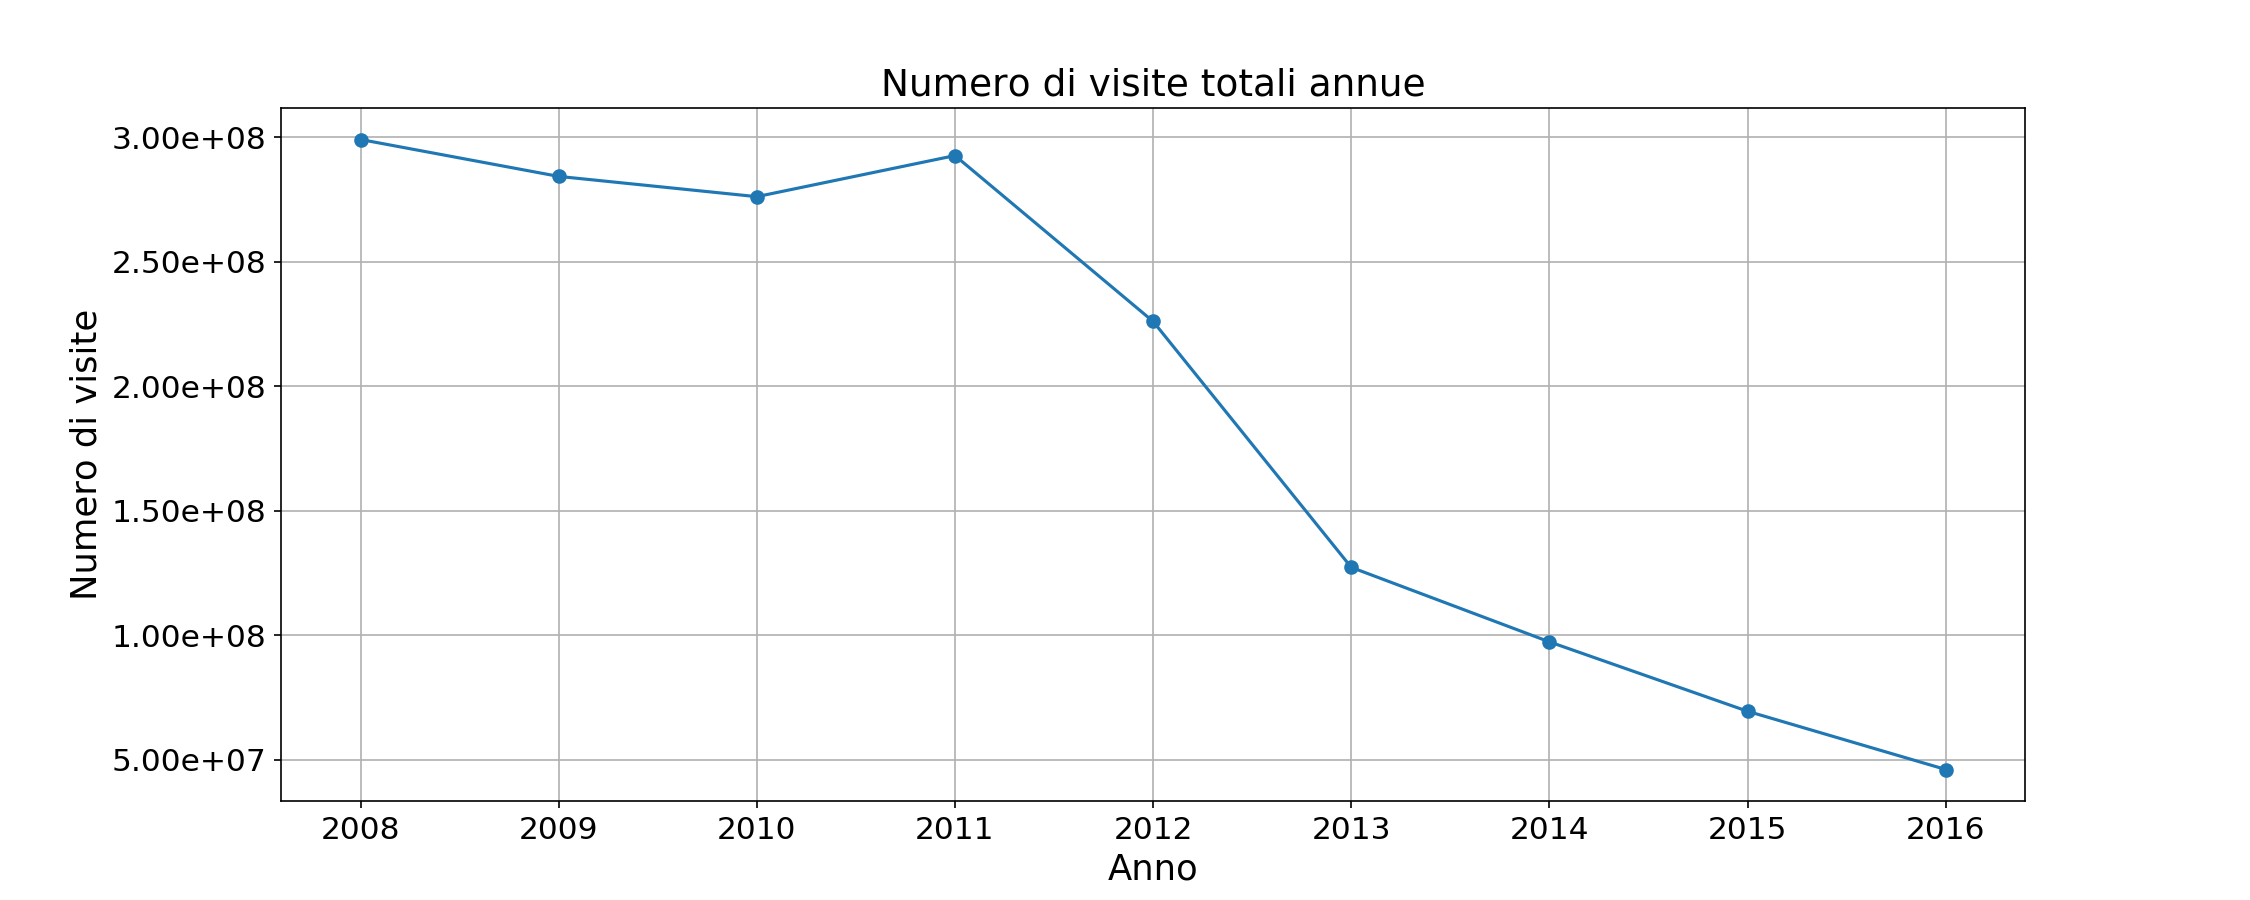
\includegraphics[width=\textwidth]{chapter_2_annual_visit}
\caption{\textit{Andamento delle visite totali annue per le categorie di Wikipedia selezionate.}}
\label{fig:ch_2_annual_visit}


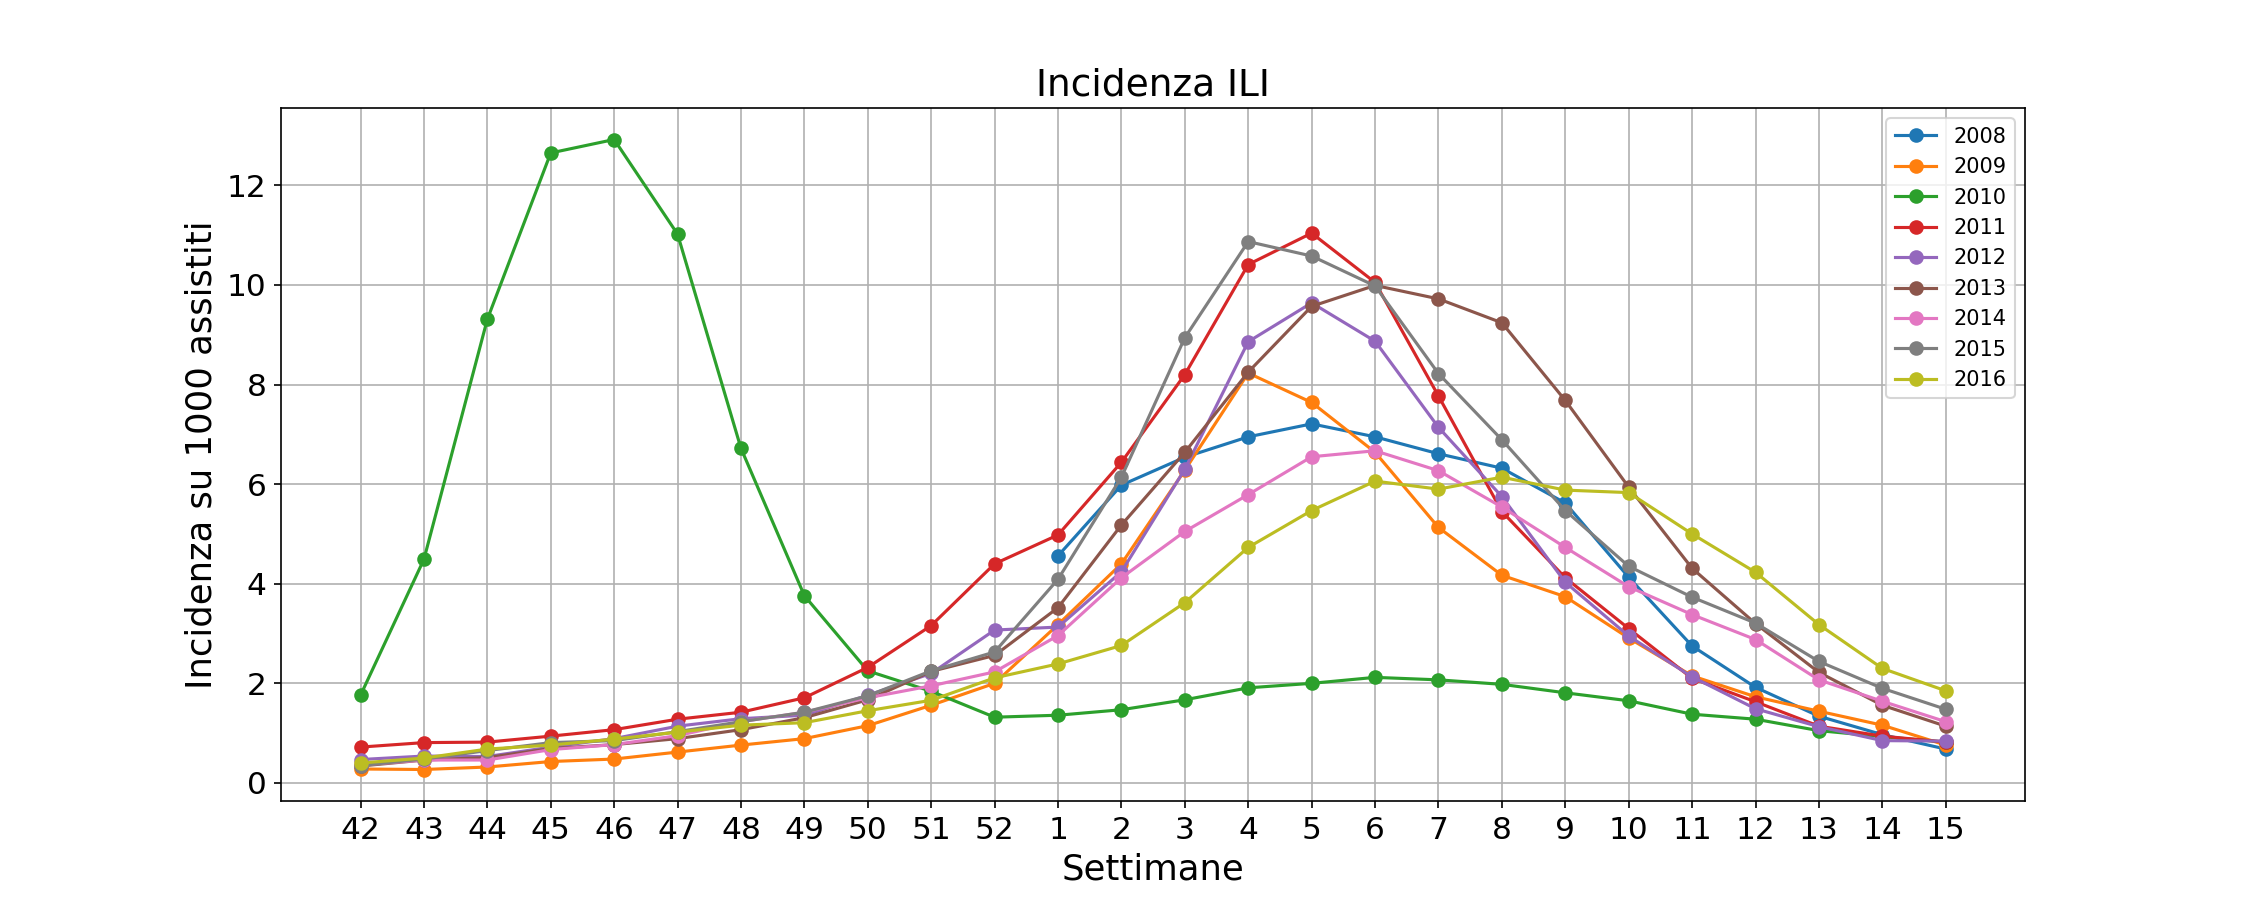
\includegraphics[width=\textwidth]{chapter_2_ILI_levels}
\caption{\textit{Livelli di incidenza della sindrome influenzale in Italia negli anni che vanno dal 2008 al 2016}}
\label{fig:ch_2_ILI_levels}

\centering

\end{figure}
\bigskip

\section{Data preprocessing}
\bigskip

Prima di poter utilizzare il dataset per allenare i vari modelli abbiamo dovuto effettuare delle attività di 
\textit{preprocessing}, per correggere alcune imperfezioni dei dati originali. Il primo problema affrontato riguarda la mancanza di dati affidabili relativamente al numero totale di visite di alcune voci di Wikipedia.
Infatti, alcune delle voci selezionate sono state create successivamente al 2007 (ad esempio nel 2010) rendendo quindi 
impossibile ottenere dati corretti sul numero di visualizzazioni settimanali prima della loro data di creazione. 
\bigskip

Per ovviare a questo problema, durante la creazione del dataset è stato effettuato un controllo sulla data di creazione di 
ogni voce (attraverso l'utilizzo di un'apposita API di Wikipedia) che permetteva di inserire dei valori identificativi $N/A
$ così da poter poi effettuare successivamente un analisi più approfondita. Ad esempio, la pagina \textit{Hepatitis_B_virus} 
è stata creata il 26 Aprile 2011, quindi, in tutti gli anni precedenti, la voce \textit{Hepatitis_B_virus} 
possiederà dei valori $N/A$. Grazie a questi indicatori, si sarebbe potuto agire su quelle voci, ad esempio 
stimando il numero di visite che quella pagina avrebbe ricevuto in quella specifica settimana (per semplicità, nel nostro 
dataset tutti i valori $N/A$ sono stati sostituiti dal valore zero).
\bigskip

Un problema successivo riguarda la diversa numerosità delle voci selezionate. Alcune voci infatti 
possiedono un volume di visite molto maggiore rispetto alle altre. Ad esempio, la pagina \textit{Raffreddore} ha una media di 
$529$ visite settimanali, contro le $2821$ di una voce come \textit{Febbre}. Nel caso di un modello lineare questo potrebbe 
causare un errato assegnamento dei valori dei pesi $\bm{\beta}$, poiché non si riesce a catturare l'importanza relativa delle 
varie feature.
\bigskip

Si è quindi applicata una tecnica di \textit{feature scaling}, che consiste nel \textit{normalizzare} i dati 
del dataset entro uno specifico range, di solito $[0, 1]$ o $[-1, 1]$, così da eliminare le differenze di numerosità (pur 
mantenendo le variazioni effettive del valore delle \textit{page view}). Nel nostro caso si è ridotto le feature nel range 
$[-1, 1]$ applicando questa formula per ogni feature:
\begin{equation}
\bm{x}' = \frac{\bm{x}-\bar{\bm{x}}}{\max(\bm{x})-\min(\bm{x})}
\end{equation} 
Dove $\bm{x}$ è il vettore contenete tutti i valori di una specifica feature, $\bar{\bm{x}}$ è la media dei valori assunti 
dalla feature, $\max(\bm{x})$ indica il massimo valore assunto da $\bm{x}$ e, rispettivamente, $\min(\bm{x})$ il minimo.
\bigskip

Alla fine, i dati per l'esperimento sono stati utilizzati nel seguente modo. Dato il dataset contenente le informazioni 
delle 9 stagioni influenzali in possesso, esso è stato diviso in modo da ottenere un dataset di training e un dataset 
di test disgiunti tra loro. Il dataset di test conterrà i valori di una sola stagione influenzale, mentre il dataset che 
verrà usato per allenare il modello conterrà le informazioni delle rimanenti. La procedura è stata eseguita 
per ogni stagione influenzale, così da simulare una valutazione per \textit{cross-validation} e così da ottenere una stima su 
come il modello si comporterà una volta allenato con tutto il dataset.
\bigskip
\newpage
